\documentclass[12pt, letterpaper]{article}
\usepackage[T1,T2A]{fontenc}
\usepackage[russian]{babel}
\usepackage[utf8]{inputenc}
\usepackage{amsmath}
\DeclareMathOperator\erf{erf}
\usepackage{listings}
\usepackage{xcolor, graphicx}
\usepackage{float}
\usepackage{tikz}
\usepackage{hyperref}
\hypersetup{
    colorlinks=true,
    linkcolor=cyan,
    filecolor=magenta,      
    urlcolor=blue,
    pdfpagemode=FullScreen,
    }

\title{Отчёт по лабораторной работе №22 по курсу “Языки и методы программирования”}
\author{Горюнов Даниил}
\begin{document}
\maketitle
\begin{description}
\item\textbf{Студент группы:} \underline{М80-108Б-22 Горюнов Даниил Владимирович, № по списку 4}    
\item\textbf{Контакты e-mail:} \underline{dania.goryunow2013@yandex.ru}
\item\textbf{Работа выполнена:} \underline{«6» апреля 2023 г.}
\item\textbf{Входной контроль знаний с оценкой:} 
\item\textbf{Преподаватель:} \underline{асп. каф. 806 Сахарин Никита Александрович}
\item\textbf{Отчет сдан} \underline{«1» апреля 2023 г.}, \textbf{итоговая оценка:}
\item\textbf{Подпись преподавателя:} \underline{\hspace{3cm}}
\end{description}
\section{Тема}
Издательская система \TeX{}.
\section{Цель работы}
Получить навыки оформления документов в издательской системе \LaTeX{}.
\section{Задание}
Оформить отчёт об изучении \LaTeX{} на \LaTeX{}.
\section{Оборудование}
\begin{description}
\item\textbf{Процессор:} Apple M1
\item\textbf{ОП:} 8192 mb
\item\textbf{SSD:} 512 Gb SSD
\item\textbf{Монитор:} Retina c диагональю 13,3 дюйма разрешение 2560×1600 пикселей (227 пикселей)
\end{description}
\section{Программное обеспечение}
\begin{description}
\item\textbf{Операционная система семейства:} MacOS
\item\textbf{Интерпретатор команд:} Visual Studio Code версия 1.76.0
\item\textbf{Текстовый редактор:} Visual Studio Code версия 1.76.0
\end{description}
\section{Идея, метод, алгоритм решения задачи}
Прочитать документацию \LaTeX{} и переписать отчет с Markdown на \LaTeX{}. tex-файл скомпилировать с помощью утилиты pdflatex.
\section{Сценарий выполнения работы}
Продемонстрируем широкий функционал \LaTeX{} на следующих примерах.
\subsection{Пример формул}
\[\cos (2\alpha) = \cos^2 \alpha - \sin^2 \alpha = 2\cos\alpha - 1 = 1 - 2\sin\alpha\]
\[A=
\begin{pmatrix}
1 & 2 & 3\\
4 & 5 & 6
\end{pmatrix}\]
\[
\lim\limits_{x \to \infty} \exp(-x) = 0
\]
\begin{figure}[h]
\centering
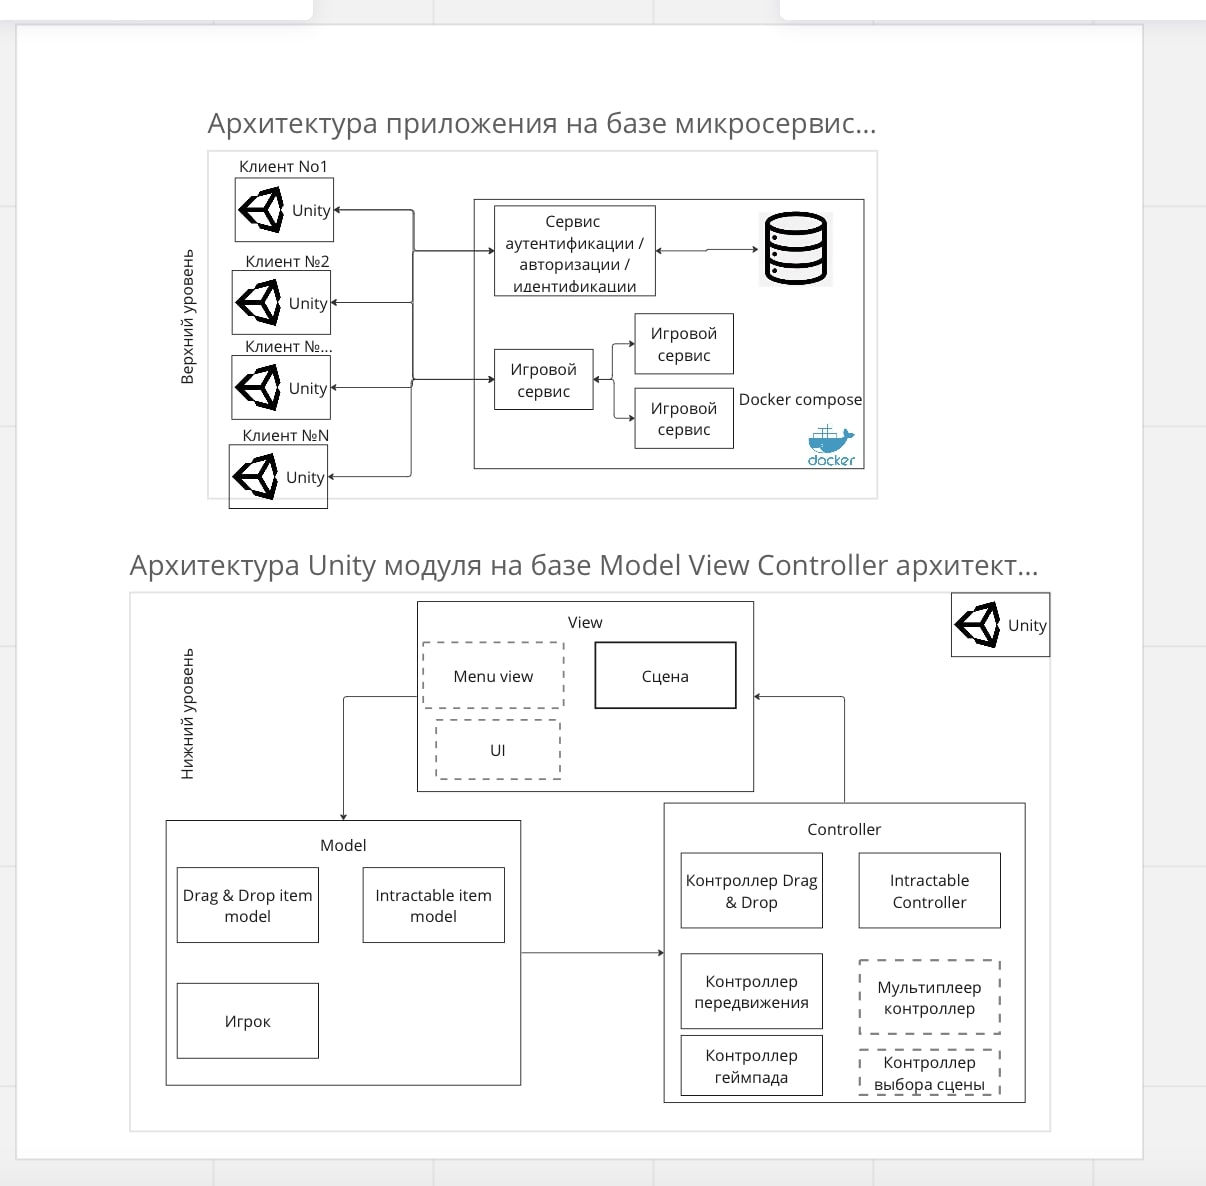
\includegraphics[width=0.9\linewidth]{p.jpg}
\caption{Это подпись к картинкам}
\label{fig:mpr}
\end{figure}
\section{Распечатка протокола}
\begin{lstlisting}[breaklines]
    This is pdfTeX, Version 3.141592653-2.6-1.40.22 (TeX Live 2021 Gentoo Linux) (preloaded format=pdflatex)
    restricted \write18 enabled.
    Output written on report.pdf (4 pages, 415766 bytes).
    Transcript written on report.log.
\end{lstlisting}  
\section{Дневник отладки}
\begin{tabular}{|c|p{1cm}|p{1.5cm}|c|p{2.5cm}|p{2cm}|p{2.25cm}|}
    \hline
    № & Лаб. или дом. & Дата & Время & Событие & Действие по исправлению & Примечание\\
    \hline
    1 & Дом. & 4.04.23 & 14:00 & Выполнение лабораторной работы & - & -\\
    \hline
\end{tabular}
\section{Замечания автора по существу работы}
\begin{itemize}
\item \href{https://codeforces.com/contest/1808/submission/199664376}{Контест (Div. 2)}
\item \href{https://codeforces.com/contest/1808/submission/200104090}{Дорешка}
\end{itemize}
\section{Выводы}
Были получены навыки оформления докладов в издательской системе \LaTeX{}. Эта система продемонстрировала свою удобность для меня и в дальнейшем будет использована вместо MS Word для оформления курсовых работ по различным предметам. \\
\flushright \textbf{Подпись студента:} \underline{\hspace{3cm}}
\end{document}

